\documentclass[tikz,border=10pt]{standalone}
\usepackage{tikz}
\usepackage{xcolor}
\usetikzlibrary{
  arrows.meta,
  positioning,
  shapes.geometric,
  shapes.misc,
  backgrounds,
  fit,
  decorations.pathmorphing,
  calc
}

%% ── Colour palette ─────────────────────────────────────────────────────────
\definecolor{titleBg}{RGB}{94,77,178}       % purple title bar
\definecolor{reprBg}{RGB}{255,250,205}      % yellow-cream: representation
\definecolor{transBg}{RGB}{255,255,255}     % white: translation
\definecolor{colearn}{RGB}{237,224,255}     % lavender: co-learning
\definecolor{fusionBg}{RGB}{250,218,221}    % pink: fusion
\definecolor{alignBg}{RGB}{224,240,255}     % light blue: alignment
\definecolor{modalA}{RGB}{221,238,255}      % light blue modality box
\definecolor{modalAbd}{RGB}{51,102,170}     % border
\definecolor{modalB}{RGB}{255,221,224}      % light red modality box
\definecolor{modalBbd}{RGB}{170,51,51}      % border
\definecolor{nodeBlue}{RGB}{136,136,255}
\definecolor{nodeRed}{RGB}{255,102,102}
\definecolor{outerBorder}{RGB}{94,77,178}

%% ── Tikz styles ─────────────────────────────────────────────────────────────
\tikzset{
  modalboxA/.style={
    draw=modalAbd, fill=modalA, line width=1.5pt,
    minimum width=1.5cm, minimum height=1.2cm,
    font=\bfseries\Large, text=modalAbd
  },
  modalboxB/.style={
    draw=modalBbd, fill=modalB, line width=1.5pt,
    minimum width=1.5cm, minimum height=1.2cm,
    font=\bfseries\Large, text=modalBbd
  },
  sectiontitle/.style={
    font=\bfseries\large, align=center
  },
  smallnode/.style={
    circle, draw, inner sep=0pt, minimum size=6pt
  },
  bluenode/.style={
    smallnode, fill=nodeBlue, draw=blue!60!black
  },
  rednode/.style={
    smallnode, fill=nodeRed,  draw=red!70!black
  },
  graynode/.style={
    smallnode, fill=gray!35,  draw=gray!60
  },
  blacknode/.style={
    smallnode, fill=black!85, draw=black
  },
  myarrow/.style={
    -{Stealth[length=5pt,width=4pt]}, line width=1.2pt, color=gray!70!black
  },
  wideArrow/.style={
    {Stealth[length=8pt,width=7pt]}-{Stealth[length=8pt,width=7pt]},
    line width=2pt, color=black!70
  },
  dashedBorder/.style={
    draw=outerBorder, line width=1.8pt, dashed, rounded corners=8pt, fill=white
  }
}

\begin{document}
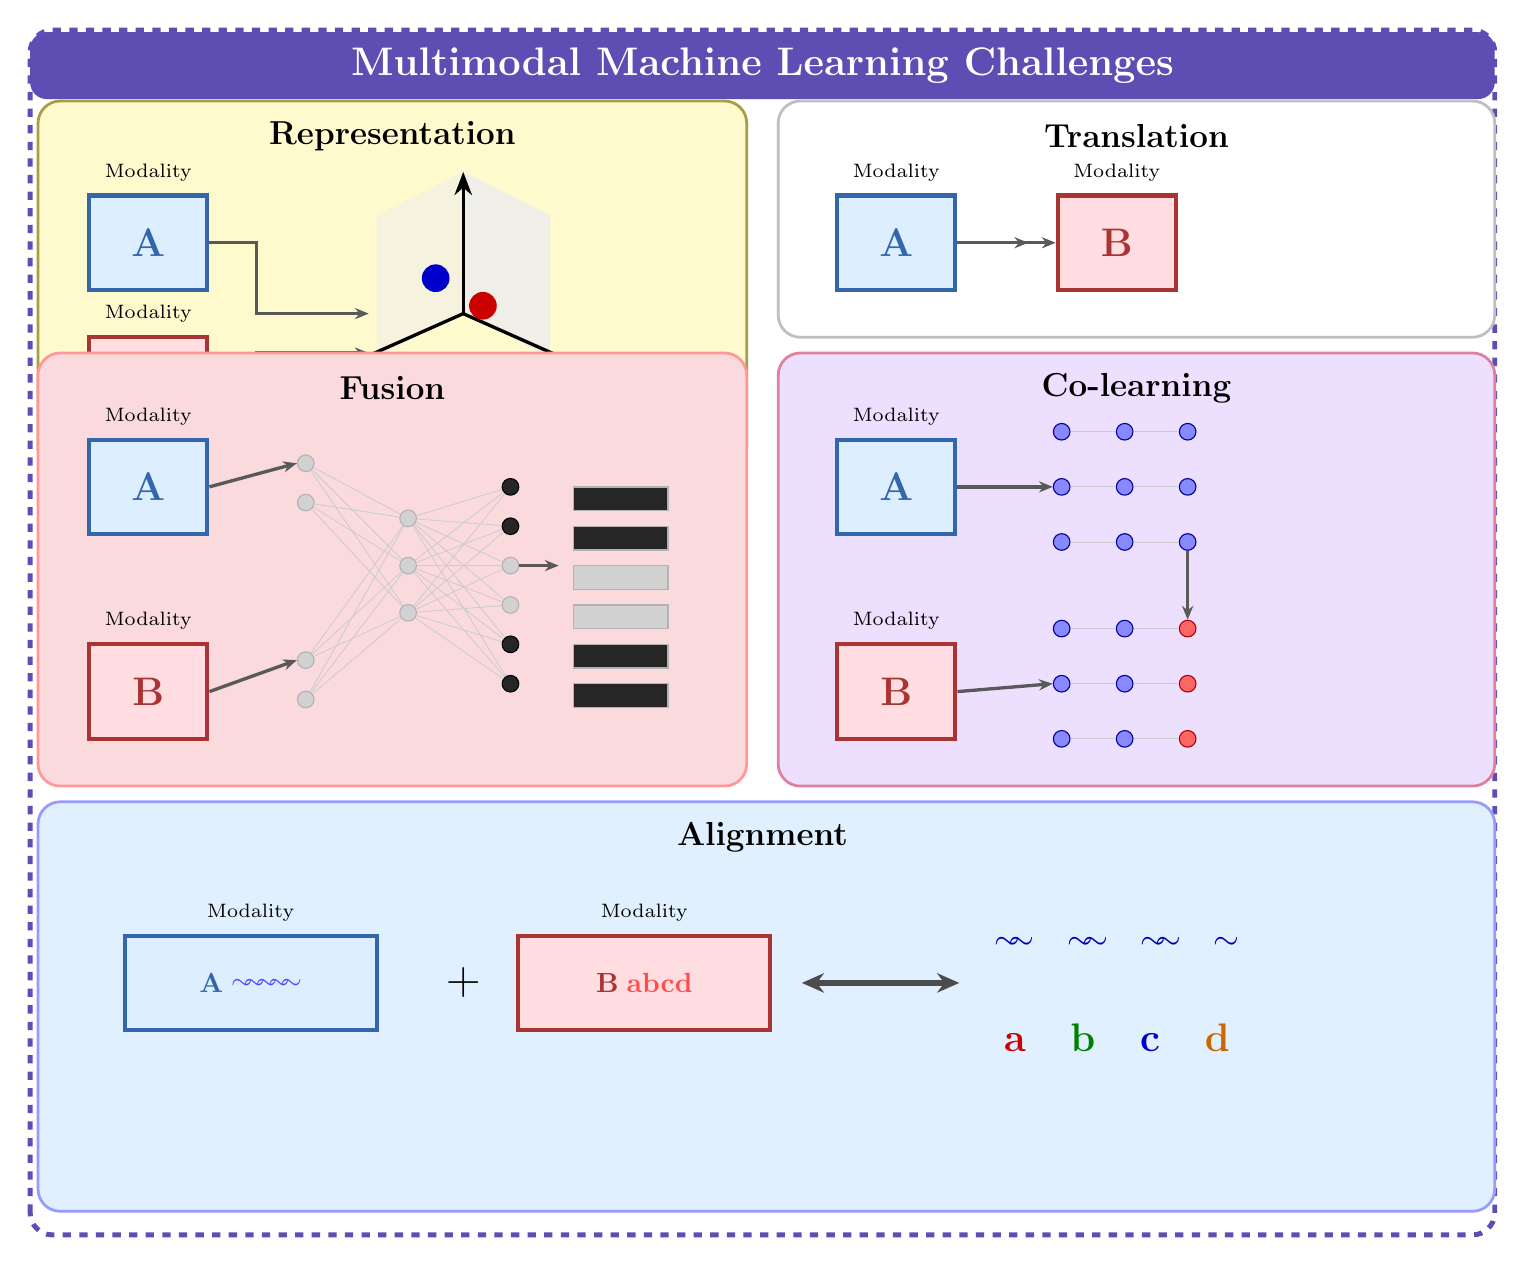
\begin{tikzpicture}[>=Stealth]

%% ════════════════════════════════════════════════════════════════
%%  OUTER FRAME + TITLE
%% ════════════════════════════════════════════════════════════════
\draw[dashedBorder] (-0.3,-14.5) rectangle (18.3,0.8);

\node[fill=titleBg, text=white, font=\bfseries\Large,
      minimum width=18.6cm, minimum height=0.85cm,
      rounded corners=6pt]
  at (9, 0.35) {Multimodal Machine Learning Challenges};

%% ════════════════════════════════════════════════════════════════
%%  SECTION 1 — REPRESENTATION  (top-left)
%% ════════════════════════════════════════════════════════════════
\begin{scope}
  \fill[reprBg, rounded corners=8pt]
    (-0.2,-4.8) rectangle (8.8,-0.1);
  \draw[draw=yellow!60!black, line width=1pt, rounded corners=8pt]
    (-0.2,-4.8) rectangle (8.8,-0.1);
  \node[sectiontitle] at (4.3,-0.55) {Representation};

  % Modality A
  \node[modalboxA] (repA) at (1.2,-1.9) {A};
  \node[font=\scriptsize, above=1pt of repA] {Modality};

  % Modality B
  \node[modalboxB] (repB) at (1.2,-3.7) {B};
  \node[font=\scriptsize, above=1pt of repB] {Modality};

  % 3-D coordinate space (parallelogram illusion via manual drawing)
  \coordinate (O)  at (5.2,-2.8);
  \coordinate (Px) at (7.0,-3.6);   % x-axis tip
  \coordinate (Py) at (5.2,-1.0);   % y-axis tip (up)
  \coordinate (Pz) at (3.4,-3.6);   % z-axis tip

  % shaded plane face
  \fill[blue!10!white, opacity=0.55]
    (O) -- ++(1.1,-0.55) -- ++(0,1.8) -- ++(-1.1,0.55) -- cycle;
  \fill[blue!10!white, opacity=0.35]
    (O) -- ++(-1.1,-0.55) -- ++(0,1.8) -- ++(1.1,0.55) -- cycle;

  % axes
  \draw[->, line width=1.2pt] (O) -- (Py);
  \draw[->, line width=1.2pt] (O) -- (Px);
  \draw[->, line width=1.2pt] (O) -- (Pz);

  % dots
  \fill[blue!80!black]  ($(O)+(-0.35,0.45)$) circle (5pt);
  \fill[red!80!black]   ($(O)+(0.25,0.10)$)  circle (5pt);

  % arrows from modality boxes to space
  \draw[myarrow] (repA.east) -- ++(0.6,0) |- ($(O)+(-1.2,0.0)$);
  \draw[myarrow] (repB.east) -- ++(0.6,0) |- ($(O)+(-1.2,-0.5)$);
\end{scope}

%% ════════════════════════════════════════════════════════════════
%%  SECTION 2 — TRANSLATION  (top-right)
%% ════════════════════════════════════════════════════════════════
\begin{scope}
  \fill[transBg, rounded corners=8pt]
    (9.2,-3.1) rectangle (18.3,-0.1);
  \draw[gray!50, line width=1pt, rounded corners=8pt]
    (9.2,-3.1) rectangle (18.3,-0.1);
  \node[sectiontitle] at (13.75,-0.55) {Translation};

  \node[modalboxA] (trA) at (10.7,-1.9) {A};
  \node[font=\scriptsize, above=1pt of trA] {Modality};

  \draw[myarrow] (trA.east) -- ++(0.9,0)
    node[midway] {};

  \node[modalboxB] (trB) at (13.5,-1.9) {B};
  \node[font=\scriptsize, above=1pt of trB] {Modality};

  \draw[myarrow] (trA.east) -- (trB.west);
\end{scope}

%% ════════════════════════════════════════════════════════════════
%%  SECTION 3 — CO-LEARNING  (right-middle)
%% ════════════════════════════════════════════════════════════════
\begin{scope}
  \fill[colearn, rounded corners=8pt]
    (9.2,-8.8) rectangle (18.3,-3.3);
  \draw[purple!50, line width=1pt, rounded corners=8pt]
    (9.2,-8.8) rectangle (18.3,-3.3);
  \node[sectiontitle] at (13.75,-3.75) {Co-learning};

  \node[modalboxA] (coA) at (10.7,-5.0) {A};
  \node[font=\scriptsize, above=1pt of coA] {Modality};

  \node[modalboxB] (coB) at (10.7,-7.6) {B};
  \node[font=\scriptsize, above=1pt of coB] {Modality};

  %% Top neural network (3 x 3 = 9 blue nodes)
  \foreach \row/\y in {1/-4.3, 2/-5.0, 3/-5.7}{
    \foreach \col/\x in {1/12.8, 2/13.6, 3/14.4}{
      \node[bluenode] (coT\row\col) at (\x,\y) {};
    }
  }
  %% Bottom neural network  (3 x 3 blue + 3 red outputs)
  \foreach \row/\y in {1/-6.8, 2/-7.5, 3/-8.2}{
    \foreach \col/\x in {1/12.8, 2/13.6}{
      \node[bluenode] (coB\row\col) at (\x,\y) {};
    }
    \node[rednode] (coBR\row) at (14.4,\y) {};
  }

  % Sparse inter-layer edges top network
  \foreach \r in {1,2,3}{
    \foreach \c in {1,2,3}{
      \foreach \cc in {1,2,3}{
        \draw[gray!40, line width=0.3pt] (coT\r1) -- (coT\r2);
        \draw[gray!40, line width=0.3pt] (coT\r2) -- (coT\r3);
      }
    }
  }
  % Sparse inter-layer edges bottom network
  \foreach \r in {1,2,3}{
    \draw[gray!40, line width=0.3pt] (coB\r1) -- (coB\r2);
    \draw[gray!40, line width=0.3pt] (coB\r2) -- (coBR\r);
  }

  % Arrows from modality boxes -> networks
  \draw[myarrow] (coA.east) -- (coT21.west);
  \draw[myarrow] (coB.east) -- (coB21.west);

  % Down arrow connecting the two networks
  \draw[myarrow] (coT33.south) -- (coBR1.north);
\end{scope}

%% ════════════════════════════════════════════════════════════════
%%  SECTION 4 — FUSION  (left-middle)
%% ════════════════════════════════════════════════════════════════
\begin{scope}
  \fill[fusionBg, rounded corners=8pt]
    (-0.2,-8.8) rectangle (8.8,-3.3);
  \draw[red!40, line width=1pt, rounded corners=8pt]
    (-0.2,-8.8) rectangle (8.8,-3.3);
  \node[sectiontitle] at (4.3,-3.75) {Fusion};

  \node[modalboxA] (fuA) at (1.2,-5.0) {A};
  \node[font=\scriptsize, above=1pt of fuA] {Modality};

  \node[modalboxB] (fuB) at (1.2,-7.6) {B};
  \node[font=\scriptsize, above=1pt of fuB] {Modality};

  %% Input layer
  \node[graynode] (fi1) at (3.2,-4.7) {};
  \node[graynode] (fi2) at (3.2,-5.2) {};
  \node[graynode] (fi3) at (3.2,-7.2) {};
  \node[graynode] (fi4) at (3.2,-7.7) {};

  %% Hidden layer
  \node[graynode] (fh1) at (4.5,-5.4) {};
  \node[graynode] (fh2) at (4.5,-6.0) {};
  \node[graynode] (fh3) at (4.5,-6.6) {};

  %% Output layer (alternating black / gray)
  \node[blacknode] (fo1) at (5.8,-5.0) {};
  \node[blacknode] (fo2) at (5.8,-5.5) {};
  \node[graynode]  (fo3) at (5.8,-6.0) {};
  \node[graynode]  (fo4) at (5.8,-6.5) {};
  \node[blacknode] (fo5) at (5.8,-7.0) {};
  \node[blacknode] (fo6) at (5.8,-7.5) {};

  % Connect input to hidden
  \foreach \i in {fi1,fi2,fi3,fi4}{
    \foreach \h in {fh1,fh2,fh3}{
      \draw[gray!40, line width=0.3pt] (\i) -- (\h);
    }
  }
  % Connect hidden to output
  \foreach \h in {fh1,fh2,fh3}{
    \foreach \o in {fo1,fo2,fo3,fo4,fo5,fo6}{
      \draw[gray!40, line width=0.3pt] (\h) -- (\o);
    }
  }

  % Arrows from modal boxes -> network inputs
  \draw[myarrow] (fuA.east) -- (fi1.west);
  \draw[myarrow] (fuB.east) -- (fi3.west);

  % Arrow from network -> classification bar chart
  \draw[myarrow] (fo3.east) -- ++(0.5,0);

  %% Output classification bars (tall rectangle, alternating fill)
  \fill[black!85] (6.6,-5.0) rectangle (7.8,-5.3);
  \fill[black!85] (6.6,-5.5) rectangle (7.8,-5.8);
  \fill[gray!35]  (6.6,-6.0) rectangle (7.8,-6.3);
  \fill[gray!35]  (6.6,-6.5) rectangle (7.8,-6.8);
  \fill[black!85] (6.6,-7.0) rectangle (7.8,-7.3);
  \fill[black!85] (6.6,-7.5) rectangle (7.8,-7.8);
  \draw[gray!60, line width=0.5pt]
    (6.6,-5.0) rectangle (7.8,-5.3)
    (6.6,-5.5) rectangle (7.8,-5.8)
    (6.6,-6.0) rectangle (7.8,-6.3)
    (6.6,-6.5) rectangle (7.8,-6.8)
    (6.6,-7.0) rectangle (7.8,-7.3)
    (6.6,-7.5) rectangle (7.8,-7.8);
\end{scope}

%% ════════════════════════════════════════════════════════════════
%%  SECTION 5 — ALIGNMENT  (bottom full-width)
%% ════════════════════════════════════════════════════════════════
\begin{scope}
  \fill[alignBg, rounded corners=8pt]
    (-0.2,-14.2) rectangle (18.3,-9.0);
  \draw[blue!40, line width=1pt, rounded corners=8pt]
    (-0.2,-14.2) rectangle (18.3,-9.0);
  \node[sectiontitle] at (9.0,-9.45) {Alignment};

  % Modality A waveform box
  \node[modalboxA, minimum width=3.2cm, minimum height=1.2cm,
        font=\normalsize] (alA) at (2.5,-11.3) {%
    \textbf{\textcolor{modalAbd}{A}}\;%
    \textcolor{blue!70}{\raisebox{1pt}{%
      $\sim\!\!\sim\!\!\sim\!\!\sim\!\!\sim$}}};
  \node[font=\scriptsize, above=1pt of alA] {Modality};

  % Plus sign
  \node[font=\LARGE\bfseries] at (5.2,-11.3) {$+$};

  % Modality B text box
  \node[modalboxB, minimum width=3.2cm, minimum height=1.2cm,
        font=\normalsize] (alB) at (7.5,-11.3) {%
    \textbf{\textcolor{modalBbd}{B}}\;%
    \textcolor{red!70}{\textbf{abcd}}};
  \node[font=\scriptsize, above=1pt of alB] {Modality};

  % Wide double arrow
  \draw[wideArrow] (9.5,-11.3) -- (11.5,-11.3);

  % Output: waveform split into 4 segments
  \node[font=\large, text=blue!70!black] at (13.5,-10.8) {%
    $\sim\!\!\sim\quad\sim\!\!\sim\quad\sim\!\!\sim\quad\sim$};

  % Colour-coded tokens underneath
  \node[font=\Large\bfseries] at (13.5,-12.0) {%
    \textcolor{red!80!black}{a}\quad
    \textcolor{green!50!black}{b}\quad
    \textcolor{blue!80!black}{c}\quad
    \textcolor{orange!80!black}{d}};
\end{scope}

\end{tikzpicture}
\end{document}
